\chapter{Обзор существующих решений}
\label{cha:ch_1}

\section{U-net}
U-net \cite{Unet} является стандартной архитектурой для сегментации данных. Она подходит для проверки идеи
использования методов глубокого обучения для сегментации скоплений. Её симметричная структура 
позволяет абстрагировать данные изображения, подаваемого на вход, в то время как skip-connection 
слои помогают увеличивать точность сегментации.\\

\section{Детекция эффекта Сюняева-Зельдовича в данных Planck}
Эта работа по общей структуре повторяет метод, описанный в \cite{Bonjean}, с некоторыми 
дополнениями, которые будут описаны далее.\\

В первую очередь, авторы статьи нормализуют данные Planck, подбирая для каждого канала параметры 
гауссианы, которая покрывает большую часть нужных данных. Таким образом сохранено изначальное 
распределение, но значения были привдены формату, который будет лучше восприниматься нейросетевой 
моделью.\\

\begin{figure}
    \center{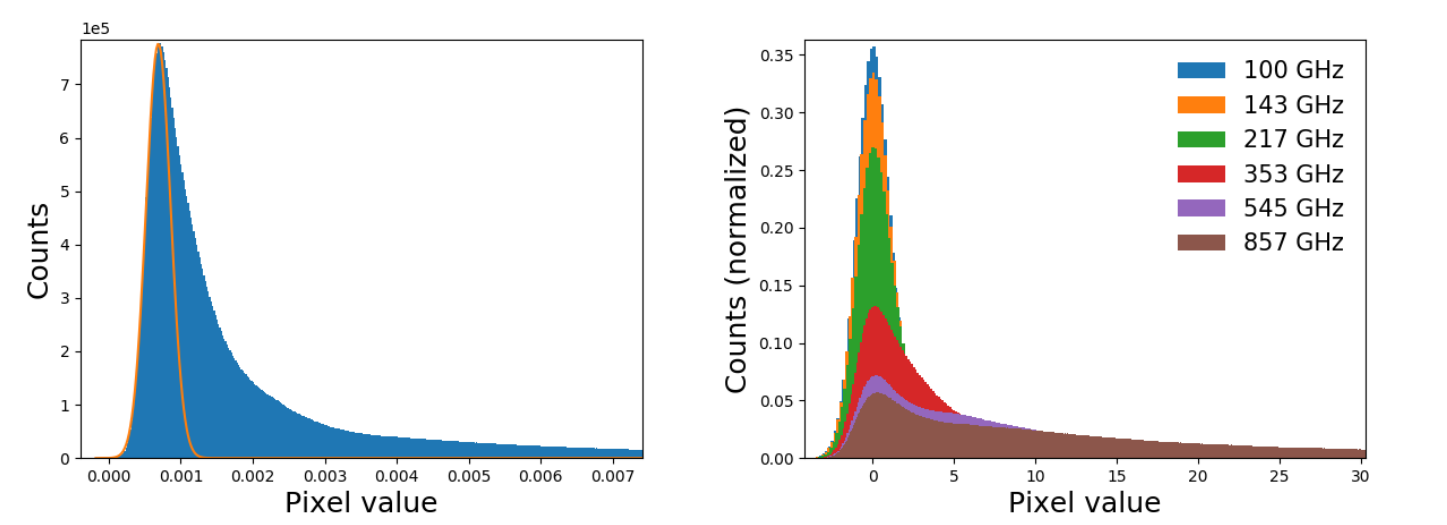
\includegraphics[width=0.6\linewidth]{planck_pre}}
    \caption{Пример подбора гауссианы для канала 353 ГГц, и сравнение распределений для всех 
        каналов после нормализации.}
\end{figure}

Далее нормализованные данные дополняются масками со скоплениями. Эти маски будут использоваться для 
обучения модели. Каждое скопление на маске отмечается как окружность диаметром $5′$.\\

Для обучения нейросетевой модели авторы статьи \cite{Bonjean} использовали следующие каталоги:\\
\begin{itemize}
    \item PSZ2\\
    \item MCXC\\
    \item RedMaPPer\\
\end{itemize}

Некоторые из этих каталогов содержат общие объекты, кроме того, обучать модель сразу на всех данных 
может оказаться нецелесообразно, поэтому списки были переработаны следующим образом:\\
\begin{itemize}
    \item planck\_z - каталог скоплений PSZ2 с известным красным смещением\\
    \item planck\_no\_z - каталог скоплений PSZ2 без красных смещений\\
    \item mcxcwp - каталог тех скоплений MCXC, что не присутствуют в PSZ2\\
    \item RM30 и RM50 - каталоги RedMaPPer\\
\end{itemize}

Основное обучение происходило на каталоге planck\_z, так как эта модель давала лучшие результаты.\\

После этого вся область неба разделяется на три части - тренировочная, валидационная и тестовая.
Для такого разбиения используется алгоритм представления данных на сфере HEALPix с параметром 
$n_{side} = 2$. В качестве валидационных выбраны пиксели $9, 38, 41$, в качестве тестовых - $6$, все 
остальные использовались для создания данных для тренировочной выборки (в статье \cite{Bonjean} 
эти пиксели нумеруются с 1, здесь с 0).
Для обучения выбирались случайные области на небе, называемые патчами. Размер патча зафиксирован: 
$64 \times 64$ пикселя в разбиении HEALPix $n_{side}=2^{11}$. Патчи выбирались так, чтобы на них 
присутствовали скопления из выбранного для обучения каталога.\\

Далее происходит обучение модели. Модель используется такая же, как и в статье: U-net с 5-ю блоками в
кодировщике, где каждый блок кодировщика содержит две свёртки $3 \times 3$ с функцией активации 
ReLU и слоём max-pooling (с увеличением количества фильтров в 2 раза). Блок кодировщика состоит из 
$2 \times 2$ upsampling свёртки (с уменьшением количества фильтров в 2 раза), конкатенации
выхода соответствующего блока из кодировщика, двух свёрток $3 \times 3$ с ReLU. Самый последний 
слой кодировщика дополняется свёрткой $1 \times 1$, кроме того, после каждой свёртки добавлен слой 
Dropout с параметром $0.2$, чтобы увеличить эффективность обучения. Для изменения весов нейросети 
использовался оптимизатор Adam с параметром $lr = 10^{-4}$. В качестве loss-функции выбрана бинарная 
кросс-энтропия. Размер батча $20$, количество эпох варьировалось от 20 до 40.\\

Для проверки результатов вся область неба сканировалась нейросетью, и на масках сегментации 
выбирались барицентры отдельных фигур, их координаты переводились в небесные, и после этого 
происходило сравнение с каталогами.\\



